\chapter{Experiments}\label{chapter:experiment}

\section{Case studies}
\paragraph{Dijkstra’s algorithm for mutual exclusion}
In this algorithm, we have a group of agents who are competing for access to a critical section.
The algorithm uses a global pointer to ensure mutual exclusion and a guarantee of progress. 
We are only checking for two things: the mutual exclusion property and whether the protocol can deadlock.
\paragraph{Dijkstra’s algorithm for mutual exclusion with a token}
The example illustrates a mutual exclusion algorithm for agents forming a ring. 
They pass around a single token as a semaphore for a critical region.
\paragraph{Other mutual exclusion algorithms}
Additionally, we also consider the mutual exclusion algorithms of Burns
, Szymanski and the standard bakery algorithm.
\paragraph{Dining philosophers}
\paragraph{Cache coherence protocols}
\paragraph{Termination detection}
\paragraph{Dining cryptographers}
\paragraph{Leader election}
\paragraph{Token passing}

\section{Dodo}
Dodo supports there interpretations (trap, siphon and flow).
Run for every system with  4 algorithms (L*, NL*, KV, RS). 
After that, it plotted the graphs to compare the learned time 
of theses algorithms.

For easier analysing, we use the library mathplot for 
plotting our graph.

\section{Results}
They represent the result of token-passing learning precess.
The color blue means that we can learn while the red one 
indicates the cases that we can not learn.
In the plotted graph we can compare the learning time of for 
algorithm.

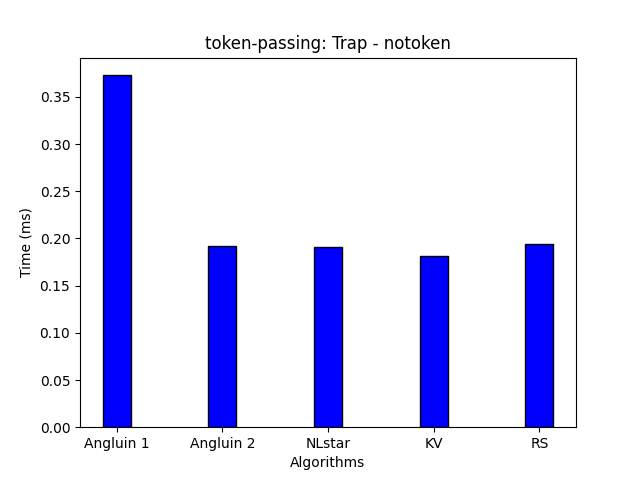
\includegraphics[scale=0.5]{figures/Trap_notoken.png}
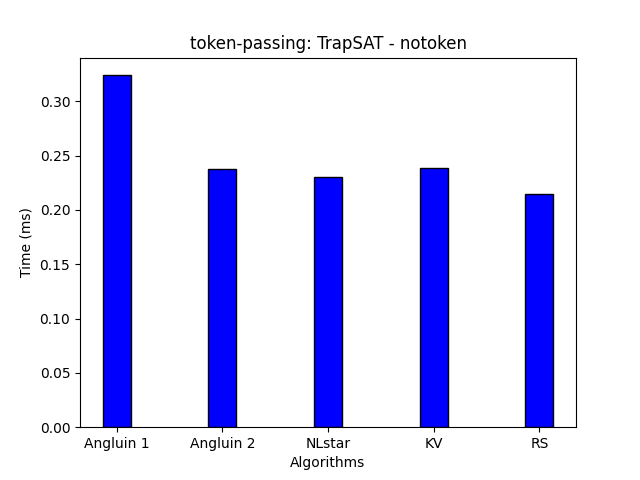
\includegraphics[scale=0.5]{figures/TrapSAT_notoken.png}

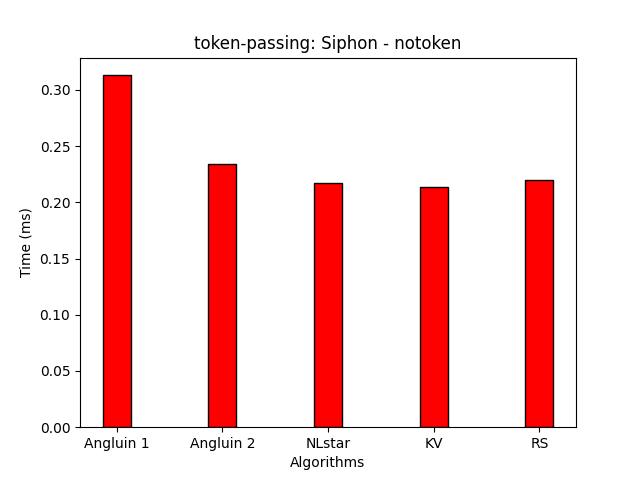
\includegraphics[scale=0.5]{figures/Siphon_notoken.png}
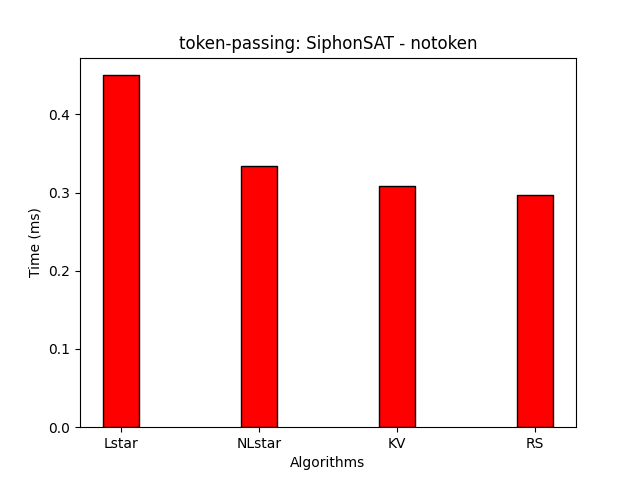
\includegraphics[scale=0.5]{figures/SiphonSAT_notoken.png}


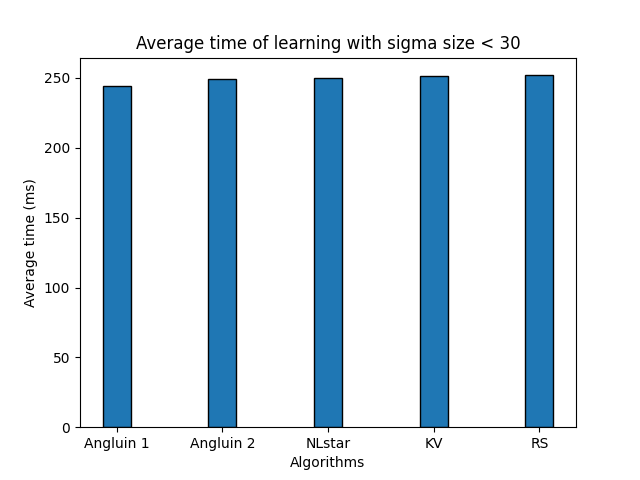
\includegraphics[scale=0.75]{figures/average_time2.png}

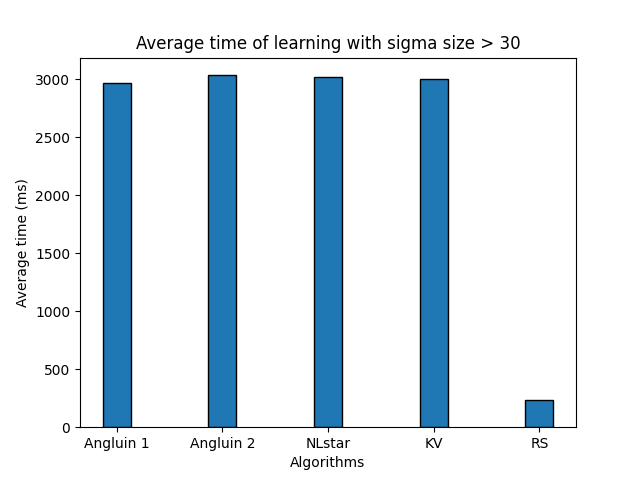
\includegraphics[scale=0.75]{figures/average_time3.png}



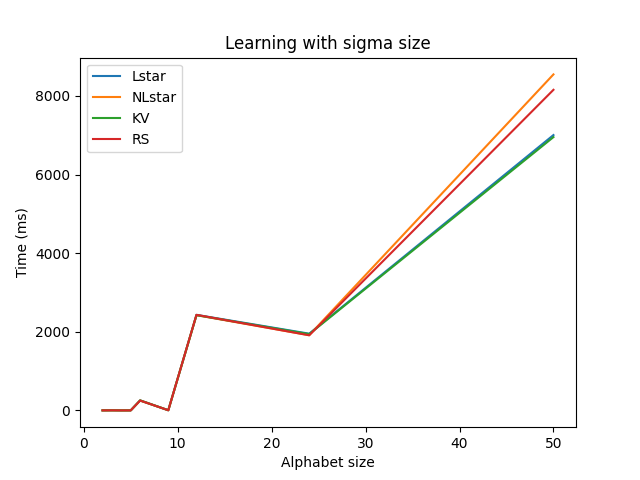
\includegraphics[scale=0.75]{figures/sigma_size.png}

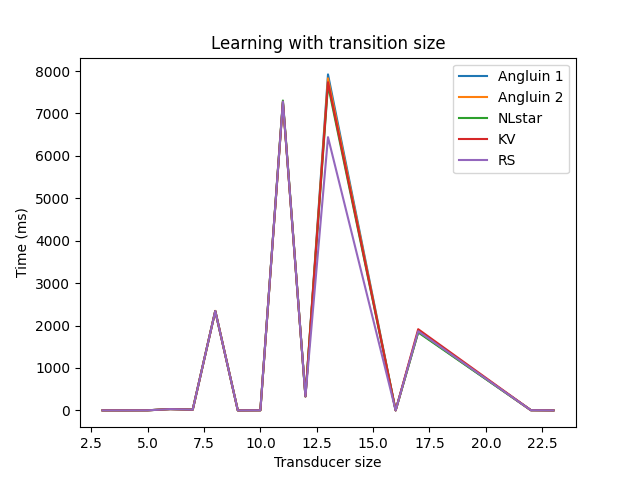
\includegraphics[scale=0.75]{figures/transition_size.png}

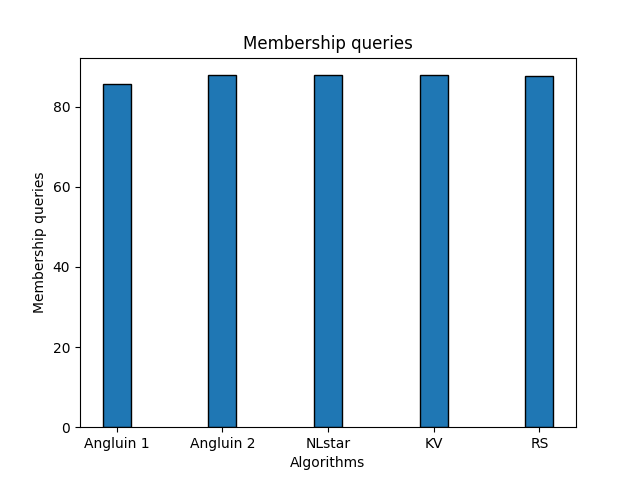
\includegraphics[scale=0.75]{figures/average_membership.png}

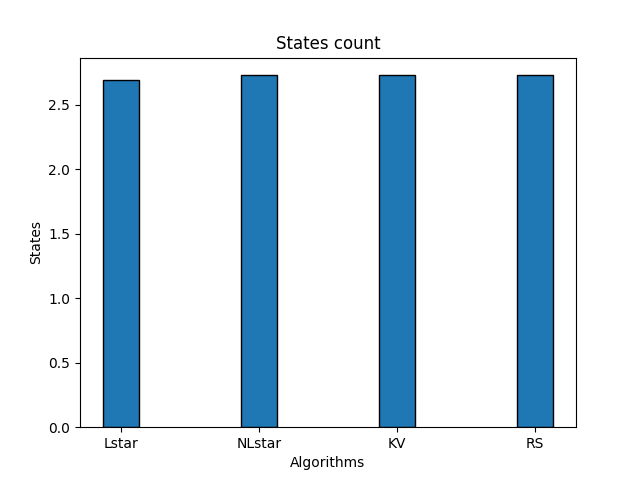
\includegraphics[scale=0.75]{figures/average_stateCount.png}